\documentclass[usenames,dvipsnames,tikz]{standalone}
\usepackage{amsmath,amssymb}
\usepackage{xcolor}
\colorlet{tBlue}{RoyalBlue!35!Cerulean}
\colorlet{tRed}{Red}
\usepackage{tikz}
\usepackage{standalone}
\begin{document}
	
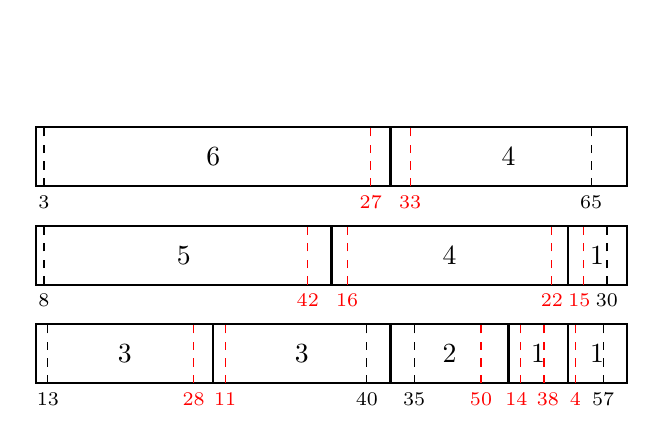
\begin{tikzpicture}
%\draw [help lines] (-1,-2) grid (8,5);
% 1=0.1, 2=0.15, 3=0.2, 4=0.25, 5=0.3
% 6 (3-27), 5 (8-42), 4 (33-65), 4 (16-22), 3 (13-28), 3 (11-40), 2 (35-50), 1 (15-30), 1 (14-38), 1 (4-57).

% BPP
\draw [thick] (0,0) rectangle (7.5,0.75);
\draw [thick] (0,1.25) rectangle (7.5,2);
\draw [thick] (0,2.5) rectangle (7.5,3.25);
\draw [thick, white] (0,3.75) rectangle (7.5,4.5);
 
% Bottom row, 3, 3, 2, 1 (13-28 X 11-40, 35-50 X 14-38 X 4-47)
\draw [thick] (2.25,0) -- (2.25,0.75);
\draw [thick] (4.5,0) -- (4.5,0.75);
\draw [thick] (6,0) -- (6,0.75);
\draw [thick] (6.75,0) -- (6.75,0.75);

\draw [dashed] (0.15,0) -- (0.15,0.75); 
\draw [dashed, tRed] (2,0) -- (2,0.75);

\draw [dashed, tRed] (2.4,0) -- (2.4,0.75);
\draw [dashed] (4.2,0) -- (4.2,0.75);

\draw [dashed] (4.8,0) -- (4.8,0.75);
\draw [dashed, tRed] (5.65,0) -- (5.65,0.75);

\draw [dashed, tRed] (6.15,0) -- (6.15,0.75);
\draw [dashed, tRed] (6.45,0) -- (6.45,0.75);

\draw [dashed, tRed] (6.85,0) -- (6.85,0.75);
\draw [dashed] (7.2,0) -- (7.2,0.75);

\node [below] at (0.15,0) {\scriptsize{13}};
\node [below] at (2,0) {\textcolor{tRed}{\scriptsize{28}}};
\node [below] at (2.4,0) {\textcolor{tRed}{\scriptsize{11}}};
\node [below] at (4.2,0) {\scriptsize{40}};
\node [below] at (4.8,0) {\scriptsize{35}};
\node [below] at (5.65,0) {\textcolor{tRed}{\scriptsize{50}}};
\node [below] at (6.1,0) {\textcolor{tRed}{\scriptsize{14}}};
\node [below] at (6.5,0) {\textcolor{tRed}{\scriptsize{38}}};
\node [below] at (6.85,0) {\textcolor{tRed}{\scriptsize{4}}};
\node [below] at (7.2,0) {\scriptsize{57}};
\node at (1.125, 0.375) {3};
\node at (3.375, 0.375) {3};
\node at (5.25, 0.375) {2};
\node at (6.375, 0.375) {1};
\node at (7.125, 0.375) {1};

% Middle row, 5, 4, 1 (8-42 X 16-22 X 15-30)
\draw [thick] (3.75,1.25) -- (3.75,2);
\draw [thick] (6.75,1.25) -- (6.75,2);
\draw [dashed] (0.1,1.25) -- (0.1,2);
\draw [dashed, tRed] (3.45,1.25) -- (3.45,2);
\draw [dashed, tRed] (3.95,1.25) -- (3.95,2);
\draw [dashed, tRed] (6.55,1.25) -- (6.55,2);
\draw [dashed, tRed] (6.95,1.25) -- (6.95,2);
\draw [dashed] (7.25,1.25) -- (7.25,2);
\node [below] at (0.1,1.25) {\scriptsize{8}};
\node [below] at (3.45,1.25) {\textcolor{tRed}{\scriptsize{42}}};
\node [below] at (3.95,1.25) {\textcolor{tRed}{\scriptsize{16}}};
\node [below] at (6.55,1.25) {\textcolor{tRed}{\scriptsize{22}}};
\node [below] at (6.9,1.25) {\textcolor{tRed}{\scriptsize{15}}};
\node [below] at (7.25,1.25) {\scriptsize{30}};
\node at (1.875, 1.625) {5};
\node at (5.25, 1.625) {4};
\node at (7.125, 1.625) {1};

% Top row, 6, 4 (3-27 X 33-65)
\draw [thick] (4.5,2.5) -- (4.5,3.25);
\draw [dashed] (0.1,2.5) -- (0.1,3.25);
\draw [dashed, tRed] (4.25,2.5) -- (4.25,3.25);
\draw [dashed, tRed] (4.75,2.5) -- (4.75,3.25);
\draw [dashed] (7.05,2.5) -- (7.05,3.25);
\node [below] at (0.1,2.5) {\scriptsize{3}};
\node [below] at (4.25,2.5) {\textcolor{tRed}{\scriptsize{27}}};
\node [below] at (4.75,2.5) {\textcolor{tRed}{\scriptsize{33}}};
\node [below] at (7.05,2.5) {\scriptsize{65}};
\node at (2.25, 2.875) {6};
\node at (6, 2.875) {4};


\end{tikzpicture}

\end{document}